% Frame: Chain-of-Thought (CoT) Prompting
\begin{frame}{Chain-of-Thought (CoT) Prompting}
  \begin{itemize}
    \item Prompting can be further improved by instructing the model to reason about the task when responding
    \begin{itemize}
      \item This is very useful for tasks that require reasoning
      \item You can combine it with few-shot prompting to get better results
      \item You can also do zero-shot CoT where exemplars are not available
    \end{itemize}
  \end{itemize}
  \vspace{0.7em}
  \begin{center}
    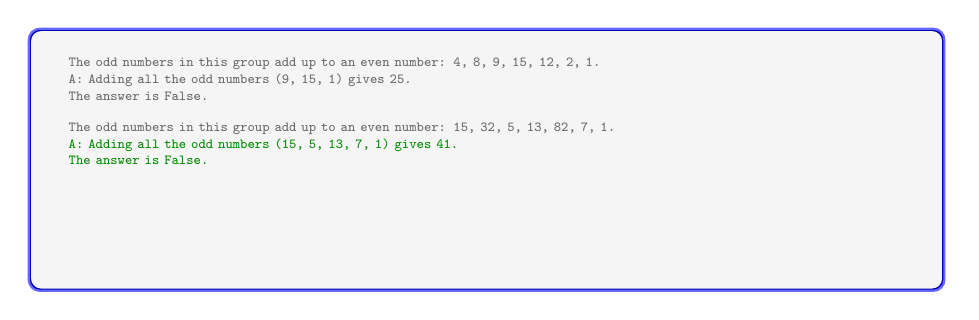
\begin{tikzpicture}
      % Outer blue rounded rectangle
      \node[
        draw=blue!70!black, 
        thick, 
        rounded corners=4pt, 
        fill=gray!8, 
        anchor=north west, 
        minimum width=11.6cm, 
        minimum height=3.3cm, 
        inner sep=0pt
      ] (cotbox) at (0,0) {};

      % First gray code block
      \node[
        anchor=north west, 
        font=\ttfamily\tiny, 
        text width=11.0cm, 
        align=left, 
        inner sep=2mm,
        text=gray!82!black
      ] at ([xshift=0.3cm, yshift=-0.17cm]cotbox.north west) {%
The odd numbers in this group add up to an even number: 4, 8, 9, 15, 12, 2, 1.\\
A: Adding all the odd numbers (9, 15, 1) gives 25.\\
The answer is False.\\[1.0em]
The odd numbers in this group add up to an even number: 15, 32, 5, 13, 82, 7, 1.\\
\textcolor{green!55!black}{A: Adding all the odd numbers (15, 5, 13, 7, 1) gives 41.}\\
\textcolor{green!55!black}{The answer is False.}
      };

      % Blue outline for clarity (ensures border matches slide)
      \draw[draw=blue!60, thick, rounded corners=4pt]
        (cotbox.north west) rectangle (cotbox.south east);

    \end{tikzpicture}
  \end{center}
  \vspace{0.25em}
  {\scriptsize
    \color{gray!75!black}
    Source: \url{https://arxiv.org/abs/2201.11903} (adapted presentation, Lady Margaret Hall, Oxford)
  }
\end{frame}

\begin{frame}{Zero-Shot CoT}
  \vspace{-0.4em}
  \begin{itemize}
    \item Involves adding \textbf{``Let's think step by step''} to the original prompt
  \end{itemize}
  \vspace{0.9em}
  \begin{center}
    \begin{tikzpicture}
      % Outer blue rounded rectangle
      \node[
        draw=blue!70!black, 
        thick, 
        rounded corners=4pt, 
        fill=gray!8, 
        anchor=north west, 
        minimum width=11.6cm, 
        minimum height=5.35cm, 
        inner sep=0pt
      ] (cotbox) at (0,0) {};

      % Top code block (vanilla prompt)
      \node[
        anchor=north west,
        font=\ttfamily\tiny,
        text width=11.0cm,
        align=left,
        inner sep=2mm,
        text=gray!82!black
      ] (prompt1) at ([xshift=0.3cm, yshift=-0.16cm]cotbox.north west) {%
\strut I went to the market and bought 10 apples. I gave 2 apples to the neighbor and 2 to the repairman. I then went and bought 5 more apples and ate 1. How many apples did I remain with?\\
\textcolor{green!55!black}{1 apples}
      };

      % Second rectangle (CoT prompt)
      \node[
        anchor=north west,
        font=\ttfamily\tiny,
        text width=11.0cm,
        align=left,
        inner sep=2mm,
        text=gray!82!black
      ] (prompt2) at ([xshift=0.3cm, yshift=-2.71cm]cotbox.north west) {%
\strut I went to the market and\hspace{1pt} bought 10 apples. I gave 2 apples to the neighbor and 2 to the repairman. I then went and bought 5 more apples and ate 1. How many apples did I remain with?\\
Let's think step by step.\\[0.3em]
\textcolor{green!55!black}{First, you started with 10 apples.}\\
\textcolor{green!55!black}{You gave away 2 apples to the neighbor and 2 to the repairman, so you had 6 apples left.}\\
\textcolor{green!55!black}{Then you bought 5 more apples, so now you had 11 apples.}\\
\textcolor{green!55!black}{Finally, you ate 1 apple, so you would remain with 10.}
      };

      % Blue outline for clarity (ensures border matches slide)
      \draw[draw=blue!60, thick, rounded corners=4pt]
        (cotbox.north west) rectangle (cotbox.south east);

      % Dashed arrow between the code blocks
      \draw[dashed, thick, draw=black!70, -{Latex[length=2.5mm,width=2.5mm]}]
        ([xshift=5.7cm, yshift=-1.04cm]cotbox.north west)
        -- ([xshift=5.7cm, yshift=-2.05cm]cotbox.north west);

    \end{tikzpicture}
  \end{center}
  \vspace{0.2em}
  {\scriptsize
    \color{gray!75!black}
    Source: \url{https://arxiv.org/abs/2201.11903} (adapted presentation, Lady Margaret Hall, Oxford)
  }
\end{frame}
